\documentclass[letterpaper,12pt,oneside]{article}
\usepackage[top=1in, left=1.25in, right=1.25in, bottom=1in]{geometry}

\usepackage[T1]{fontenc}
\usepackage[utf8]{inputenc}
\usepackage[spanish,es-nodecimaldot,es-tabla]{babel}
\usepackage{caption, subcaption} %figuras
\usepackage{graphicx}
\usepackage{array}
\usepackage{tikz}
\usepackage{imakeidx}
\usepackage{biblatex}
\addbibresource{protocolo.bib}
\usepackage{float}
\usepackage{verbatim}

\graphicspath{{./figs/}}
\usepackage{setspace}
%\usepackage[round]{natbib}

\addto\captionsspanish{\renewcommand{\contentsname}{Contents}}
\addto\captionsspanish{\renewcommand{\figurename}{Figure}}
\begin{document}
%\frontmatter
\begin{titlepage}
		\setlength{\parindent}{0pt} \setlength{\parskip}{0pt}
	
		\begin{center}
			\vfill 
			
			\begin{minipage}{\textwidth}
				
				\newcolumntype{V}{>{\centering\arraybackslash} m{.17\textwidth} }
				\newcolumntype{C}{>{\centering\arraybackslash} m{.56\textwidth} }
				
				\begin{center}
					
\includegraphics[width=4.5cm]{UNAM_LOGO2.png}	
				\end{center} 	
				\begin{center}
					\Huge\textbf{Universidad Nacional Autónoma de México}
				\end{center} 
				
			\end{minipage}
				
			\vfill
			
			\begin{minipage}{0.7\textwidth}
				\begin{center}
					\large Ingeniería en Computación
				\end{center}
			\end{minipage}
			% 
			\begin{center}
				%\medskip \rule{.9\textwidth}{2pt}
				\vfill
				\large Compilers
				%{\Large \bfseries  \title   }
				
				%\medskip \rule{.9\textwidth}{2pt}
			\end{center}
			
			\begin{center}
				\vspace*{1cm}
				{\huge Lexical Analyzer}\\
				\vspace*{1cm}
				
				%PRESENTA:\\ \medskip
				\begin{center}
					STUDENTS: \\
					\large 321184995\\
                    \large 321331656\\
                    \large 321058526\\
                    \large 424138220\\
                    \large 320560154
				\end{center}
				
				\bigskip
				
				Group: \\
				\#05\\
				%Coadvisors
				Semester: \\
                2026-II
			\end{center}
			
			\vfill
			
			\begin{center}
				{México, CDMX. 15 March 2025}\\
			\end{center}
			\cleardoublepage
		\end{center}
	\end{titlepage}
 
\tableofcontents
\clearpage
    
%\mainmatter

\section{Introduction} %

%Este apartado debe abordar los siguientes puntos:
Compilers are an important tool for computer programming; they are computer programs used to transform high-level source code into low-level target code that the processor can execute directly. 
\\ \\
The compiler consists of phases, these are Lexical Analysis, Syntax Analysis, Semantic Analysis, Intermediate Code Generation, Code Optimization, and Target Code Generation. For the purposes of the present report, we will focus only on the lexical analysis phase, whose function is to examine the source code of a program and divide it into basic units called tokens. These tokens represent significant elements of the language, such as reserved words, identifiers, operators, constants, and punctuation marks.
\\ \\
However, processing code written in a compiled programming language needs a program that identifies and classifies each element. Without it, this compilation process could not be done.
\\ 
Hence the need arises for a lexical analyzer that can read a line of code and automatically separate it into lexemes and classify them according to the corresponding token type.
\\ \\
Being the first phase of the compilation process, it carries significant weight as it builds the foundation for the subsequent phases. Its importance lies in the ability to simplify syntactic complexity, optimizing performance by eliminating irrelevant elements, such as whitespace and comments, and serving as the first barrier for error detection.
\\ \\
Understanding its operation is essential as it is a requirement for language design and for our education as computer engineers. By understanding the operation of this phase, we will gain a richer view on how information is processed, allowing us to improve our coding skills, facilitating technical debugging, and understanding the basics of security in data validation
\\ \\
The objective of the project is developing a lexical analyzer capable of processing a text input representing source code and performing an automatic identification of the different elements that compose it, separating the elements of the language and determining whether they correspond to keywords, identifiers, punctuation marks, operators, constants, or character strings. In this way, the program will generate a structured representation of the information found in the code.
\\ \\
Finally, the goal is developing a system that not only correctly identifies each of the tokens present in the input, but also provides clear information about the classification of these elements and the total number of tokens detected, thus allowing a practical understanding of the functioning of lexical analysis within the compilation process.

\begin{comment}
\begin{itemize}
    \item \textbf{Planteamiento del problema.} Se hace una descripción del problema a resolver.
    \item \textbf{Motivación.} Se describe porqué es necesario dar solución al problema.
    \item \textbf{Objetivos.} Lo que se se espera obtener de darle solución al problema.
\end{itemize}
\end{comment}

\section{Theoretical Framework}
The lexical analysis process is just one phase of a larger process called a compiler, a computer program used to transform high-level source code into low-level target code that the processor can execute directly.
\\ \\
The first phase of the compiler is precisely lexical analysis. The lexical analyzer takes the source code as input, reads its characters and groups them into meaningful units called tokens, along with a terminal symbol that is used for syntax analysis decisions. A token represents a lexical category within a programming language, such as keywords, identifiers, operators, constants, or punctuation marks. An input sequence that forms a token is called a lexeme; therefore, the lexical analyzer isolates the syntax analyzer from the representation of tokens through lexemes.
\\ \\
To perform this recognition, lexical analyzers use pattern identification mechanisms that allow classifying each fragment of the input text. These patterns are usually described using regular expressions, which formally define how certain language elements can be formed.
\\ \\
The main function of the lexical analyzer is to scan the program and group characters into lexemes to later be classified as tokens. These are then sent to the next phase of the compiler, which is the syntax analyzer, to verify that the sequence of tokens complies with the grammatical rules of the language.
\\ \\
The lexical analyzer is also responsible for eliminating whitespace (spaces, tabs, and line breaks) or comments within expressions, so that the syntax analyzer does not have to consider them, avoiding the need to modify the grammar.
\\
We can observe that the lexical analyzer functions as a filter that organizes the program's information before further analysis.~\cite{aho2006compilers}
\\

\begin{comment}
Son los conceptos aplicados, principalmente los vistos en clase, con los que se va a dar solución al problema, explicados de forma concreta, ya sea con su interpretación personal o bien con referencias bibliográficas sólidas.~\cite{10.5555/576122} 
\end{comment}

\section{Development}

The initial CFG proposition is\\
G = (V, $\Sigma$, P, S)\\
\\
V = \{
Program, Function, StatementList, Statement, Declaration, Type, VarList, Var, Assignment, printf, ReturnLine, Expression, Term, Factor, Value, String
\}
\\\\
 $\Sigma$ =  \{
 int, float, double, main, printf, return, id, int\_literal, 
 float\_literal, +, -, *, /, =, ,, ;, (, ), {, }, "text", "%d\n"
    \} \\\\

$P = $ \\
Program $\rightarrow$ StatementList | Function \\
Function $\rightarrow$ int main() \{ StatementList ReturnLine \} \\
StatementList $\rightarrow$ Statement StatementList | Statement \\
Statement $\rightarrow$ Declaration ; $|$ \hspace{0.5cm} Assignment ;   $|$ \hspace{0.5cm} Printf ;\\
Declaration $\rightarrow$ Type VarList \\
Type $\rightarrow$ int | float | double \\
VarList $\rightarrow$ Var | Var , VarList \\
Var $\rightarrow$ id | id = Value \\
Assignment $\rightarrow$ id = Expression \\
Printf $\rightarrow$ printf ( String ) $|$ \hspace{0.5cm} printf ( String , Expression ) \\
ReturnLine $\rightarrow$ return Value ; \\
Expression $\rightarrow$ Expression + Term $|$ \hspace{0.5cm} Expression - Term $|$ \hspace{0.5cm} Term \\
Term $\rightarrow$ Term * Factor $|$ \hspace{0.5cm} Term / Factor $|$ \hspace{0.5cm} Factor \\
Factor $\rightarrow$ id | Value \\
Value $\rightarrow$ int\_literal | float\_literal \\
String $\rightarrow$ string\_literal
\\ \\
S = \{Program\} \\\\

It can form basic texts, but there is left recursion present in some rules. We'll apply this rule to the productions with left recursion
\\\\
A $\rightarrow$ $\alpha$A|B \\
Transforms into \\
A $\rightarrow$ BA'\\
A' $\rightarrow$ $\alpha$A'|$\epsilon$\\

And left factoring with this one\\
A $\rightarrow$ $\alpha$$B_1$|$\alpha$$B_2$\\
Transforms into \\
A $\rightarrow$ $\alpha$A'\\
A' $\rightarrow$ $B_1$|$B_2$\\

\noindent

The production rules end up as:\\\\
Program $\rightarrow$ StatementList | Function \\
Function $\rightarrow$ int main() \{ StatementList ReturnLine \} \\
StatementList $\rightarrow$ Statement StatementList' \\
StatementList' $\rightarrow$ Statement StatementList' | $\epsilon$ \\
Statement $\rightarrow$ Declaration ; $|$ \hspace{0.5cm} Assignment ; $|$ \hspace{0.5cm} Printf ; \\
Declaration $\rightarrow$ Type VarList \\
Type $\rightarrow$ int | float | double \\
VarList $\rightarrow$ Var VarList' \\
VarList' $\rightarrow$ , Var VarList' | $\epsilon$ \\
Var $\rightarrow$ id Var' \\
Var' $\rightarrow$ = Value | $\epsilon$ \\
Assignment $\rightarrow$ id = Expression \\
Printf $\rightarrow$ printf ( String Printf' ) \\
Printf' $\rightarrow$ , Expression | $\epsilon$ \\
ReturnLine $\rightarrow$ return Value ; \\
Expression $\rightarrow$ Term Expression' \\
Expression' $\rightarrow$ + Term Expression' $|$ \hspace{0.5cm} - Term Expression' $|$ \hspace{0.5cm} $\epsilon$ \\
Term $\rightarrow$ Factor Term' \\
Term' $\rightarrow$ * Factor Term' $|$ \hspace{0.5cm} Factor Term' $|$ \hspace{0.5cm} $\epsilon$ \\
Factor $\rightarrow$ id | Value \\
Value $\rightarrow$ int\_literal | float\_literal \\
String $\rightarrow$ string\_literal
\\\\
For the implementation of the lexical analyzer, the Python programming language was chosen. The development of the program was designed in such a way that the responsibilities of the program could be separated, facilitating the organization of the analysis. The overall application of the program mainly consists of three modules: the main execution module, the module responsible for lexical analysis, and the module that contains the token pattern table. \\ \\
In the main module, the interaction with the user and the overall control of the program are carried out. This is where a menu is displayed allowing the user to choose between two options: analyzing code from a file or analyzing code entered through the terminal. Once either option is selected, the program verifies that there is user input or, in the case of a file, that the file exists. Once this is confirmed, the program accesses the corresponding content and sends it to the next module responsible for performing the lexical analysis. \\ \\
Once the user-program interaction is completed, the module responsible for lexical analysis receives the content provided by the user, and subsequently the main token recognition procedure is implemented. This module contains several functions responsible for processing the code and generating the corresponding tokens. Each function is essential to achieve a proper analysis. \\
The analizearchive function is responsible for performing the analysis when the user provides the code through an external file. This function opens the file specified by the user, reads its entire content, and sends it to the internal procedure that performs the lexical analysis. At the same time, this function handles possible errors related to file reading, such as the nonexistence of the specified path or problems during file opening. \\
The analizeterminal function performs the analysis when the user enters the code directly through the terminal. In this case, the function receives a text string provided by the user and sends it to the internal procedure that performs the content analysis. Its purpose is to facilitate the quick evaluation of code fragments without the need to use external files. \\
The main token recognition process is carried out within the \_analizar\_contenido function. This function receives the text to be analyzed and the source from which that content originates. During execution, the program sequentially scans the input text, maintaining control over the current position within the code, as well as the line and column where each element is located. This allows the precise identification of the location of each token within the program. \\
While scanning the received content, the function compares the sequence of characters with the different patterns defined in the token table. These patterns are represented using regular expressions that allow the recognition of the different lexical categories of the language. When a match is detected between the analyzed text and one of the patterns, the program classifies the corresponding fragment as a token of the indicated type, registers it in an internal list, and continues analyzing the rest of the content. This list is used to store the recognized tokens, where in addition to displaying them along with their classification, the total number of detected tokens is calculated. \\
If the analyzer encounters a character that does not match any of the defined patterns, the system reports a lexical error indicating the invalid character and the exact position where it was detected. This allows the identification of possible errors in the analyzed source code. \\ \\
The file that defines the lexical patterns of the analyzer contains the structure that describes the rules used to recognize each type of token within the source code. This component functions as a lexical table, in which the patterns used to identify the different categories of language elements are specified. \\
The table is composed of pairs formed by a recognition pattern and its associated token type. These patterns are defined using regular expressions, which allow the formal description of the character sequences that correspond to each lexical category. This mechanism enables the analyzer to identify various types of elements present in the code during the analysis process. \\
The table includes reserved words corresponding to terms that belong to the programming language and that have a specific meaning within the language syntax. Identifiers are also defined, representing names assigned by the programmer to variables, functions, or other elements of the program. Patterns for recognizing constants are also included, which represent literal values within the code. Another important category corresponds to operators, which represent symbols used to perform operations within the language. Additionally, punctuation symbols are included, which delimit structures within the program, such as parentheses, braces, brackets, commas, and semicolons.
The table also includes patterns intended to recognize comments and whitespace. However, these elements do not generate tokens during the analysis since they are not part of the syntactic structure that will be processed by later stages of the compiler. \\
Finally, the module calculates the total number of token types defined within the table, excluding those patterns that correspond to ignored elements such as comments or whitespace. This information makes it possible to determine the variety of lexical categories that the analyzer is capable of recognizing during its execution.\\ \\
To verify the correct functioning of the lexical analyzer, several tests were performed using different code fragments as input. This allowed us to evaluate the program’s ability to identify the various tokens defined in the lexical table. \\
One of the tests performed consisted of entering a code string that contains a function call for printing and a variable declaration. The following text represents the input used: 
\begin{center}
\begin{minipage}{0.5\textwidth} 
\begin{verbatim}
printf("This is an example"); 
int a = 10;
\end{verbatim}
\end{minipage}
\end{center}
During the analysis process, the program identified and classified the different elements according to their lexical category. The detected tokens included identifiers, string constants, assignment operators, punctuation symbols, and reserved words.\\
As a result, the program produced a list of tokens representing the sequence of lexical elements found in the input. Additionally, the system reported the total number of identified tokens, allowing verification that all components of the code were correctly recognized by the analyzer.\\
Additionally, tests were performed by entering the code directly through the program’s terminal. In this case, the system allowed multiple lines of code to be entered until the user indicated the end of the input. Afterwards, the analyzer processed the entered content and displayed the detected tokens along with their corresponding classification. \\
The tests performed confirm that the lexical analyzer was able to process both external files and inputs manually entered by the user, correctly identifying the different types of tokens defined within the system.

\begin{comment}
    Es la descripción de la implementación realizada en el lenguaje de programación, así como las pruebas realizadas para obtener los resultados. Es importante resaltar lo siguiente:

\begin{itemize}
    \item No se debe mostrar código, solo describir funciones o la aplicación de los conceptos teóricos.
    \item Las pruebas es describir las entradas ingresadas y las salidas obtenidas.
\end{itemize}
\end{comment}

\section{Results}
This section will present the results obtained from testing the program. This time, you have the option to implement up to 3 versions Simple Lexer (Standard Output), Enhanced Lexer (Formatted Output) and Professional Lexer (RPLY Implementation).\\
\begin{figure}[H]
    \centering
    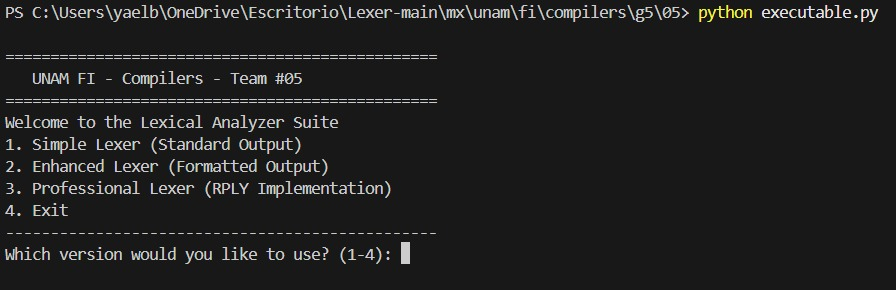
\includegraphics[width=0.8\textwidth]{fig1.png}
    \caption{}
    \label{fig:mi_imagen}
\end{figure} 
The figure above represents the start of the lexical analyzer's execution. As you can see, three options appear, as mentioned before. \\
We will begin with the first option in each case.\\
\begin{figure}[H]
     \centering
     % Primera subfigura
     \begin{subfigure}[b]{0.45\textwidth}
         \centering
         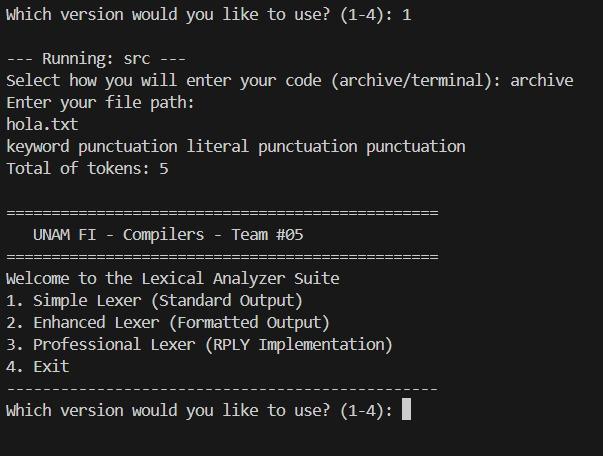
\includegraphics[width=\textwidth]{fig2.png}
         \caption{}
         \label{fig:izq}
     \end{subfigure}
     \hfill % Esto crea un espacio elástico entre las dos imágenes
     % Segunda subfigura
     \begin{subfigure}[b]{0.45\textwidth}
         \centering
         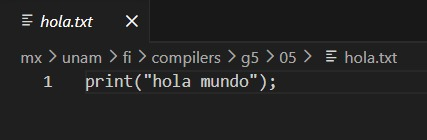
\includegraphics[width=\textwidth]{fig3.png}
         \caption{}
         \label{fig:der}
     \end{subfigure}
     \caption{}
     \label{fig:comparacion}
\end{figure} 
The operation of Simple Lexer is shown using a file as input (a). The contents of the file hola.txt are also shown (b).\\
Now, using the same Simple Lexer, we will use the terminal as input.\\ 
\begin{figure}[H]
    \centering
    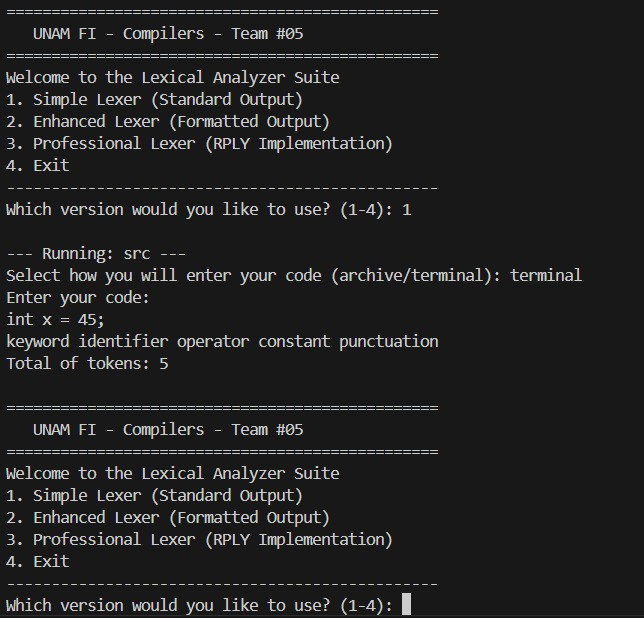
\includegraphics[width=0.5\textwidth]{fig4.png}
    \caption{}
    \label{fig:mi_imagen}
\end{figure} 
As you can see in the image, we add the following entry: 
\begin{minipage}{0.6\textwidth} 
\begin{verbatim}
int x = 45;
\end{verbatim}
\end{minipage}\\
And we obtain the lexical analysis as output.\\ \\
Now we will use the Enhanced Lexer version and follow the same protocol as before (first we'll try with a file and then with the terminal).\\
\begin{figure}[H]
     \centering
     % Primera subfigura
     \begin{subfigure}[b]{0.45\textwidth}
         \centering
         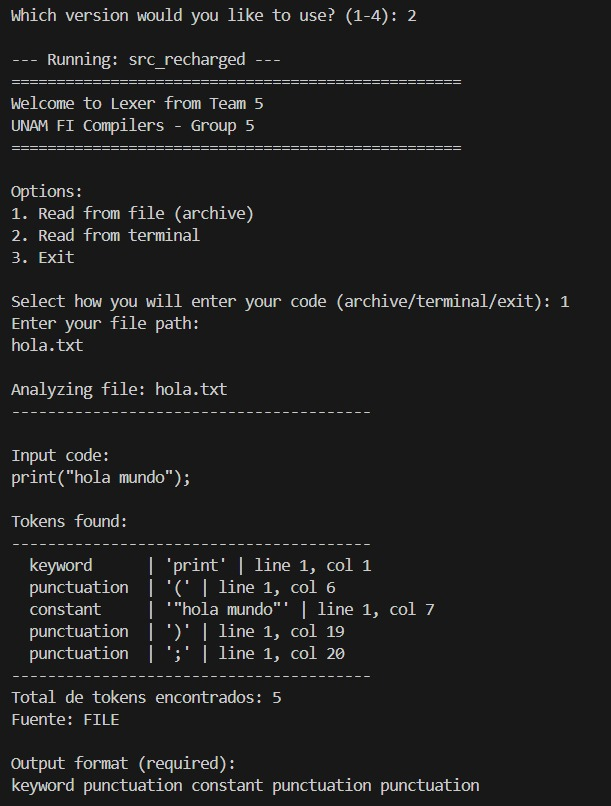
\includegraphics[width=\textwidth]{fig5.png}
         \caption{}
         \label{fig:izq}
     \end{subfigure}
     \hfill % Esto crea un espacio elástico entre las dos imágenes
     % Segunda subfigura
     \begin{subfigure}[b]{0.45\textwidth}
         \centering
         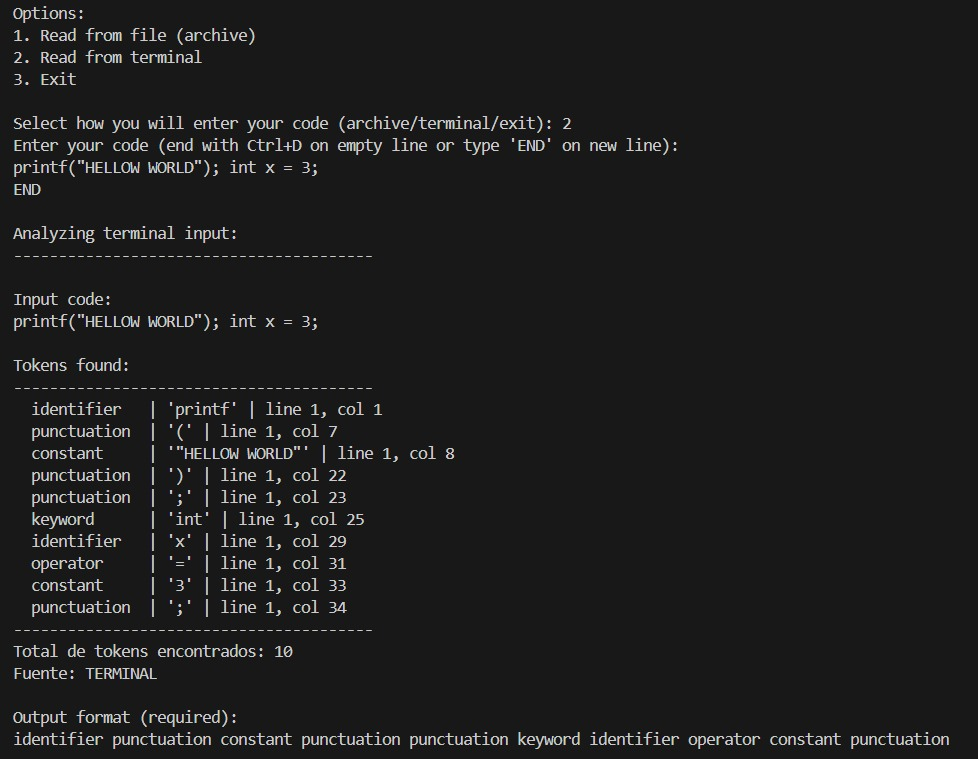
\includegraphics[width=\textwidth]{fig6.png}
         \caption{}
         \label{fig:der}
     \end{subfigure}
     \caption{}
     \label{fig:comparacion}
\end{figure} 
Image (a) shows a file used as input (Figure 2.b) for the lexical analyzer version two. Similarly, image (b) shows the input from the terminal for the lexical analysis process. The output displays the token count and its classification. \\ \\
Once the results for version 2 are finalized, we proceed to show the operation with version 3 Professional Lexer, both with a file and with the terminal.\\
\begin{figure}[H]
     \centering
     % Primera subfigura
     \begin{subfigure}[b]{0.45\textwidth}
         \centering
         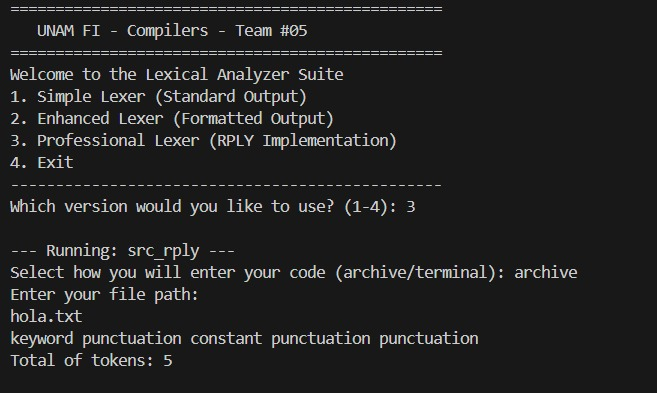
\includegraphics[width=\textwidth]{fig7.png}
         \caption{}
         \label{fig:izq}
     \end{subfigure}
     \hfill % Esto crea un espacio elástico entre las dos imágenes
     % Segunda subfigura
     \begin{subfigure}[b]{0.45\textwidth}
         \centering
         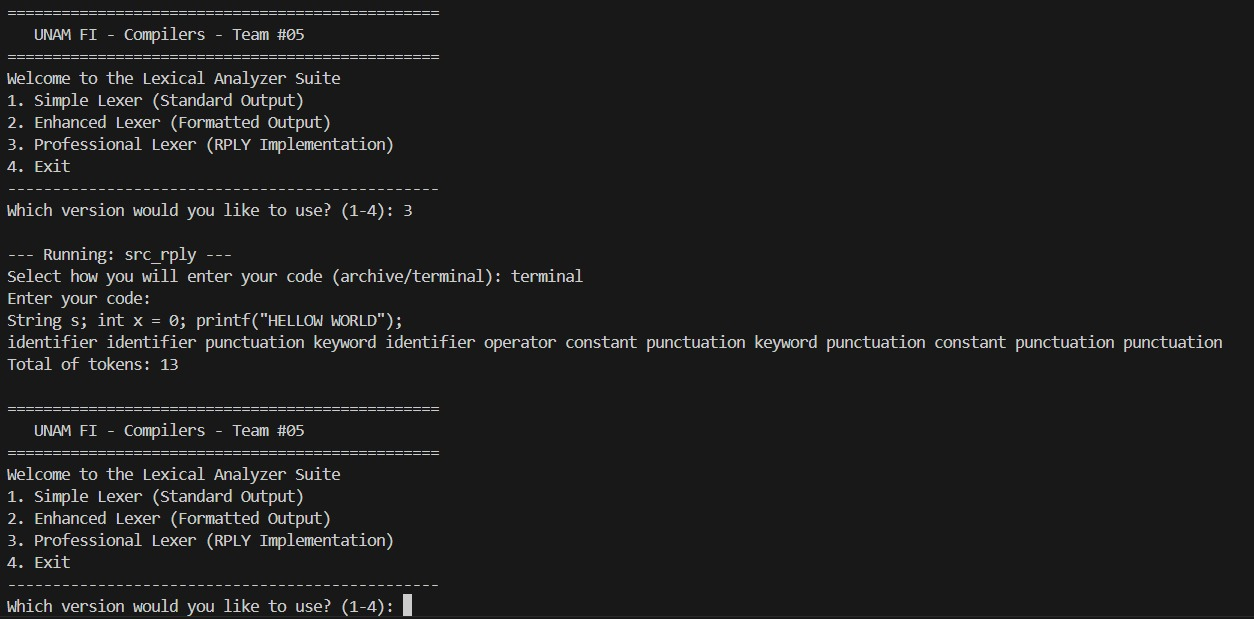
\includegraphics[width=\textwidth]{fig8.png}
         \caption{}
         \label{fig:der}
     \end{subfigure}
     \caption{}
     \label{fig:comparacion}
\end{figure} 
Image (a) shows a file used as input (Figure 2.b) for the lexical analyzer version three. Similarly, image (b) shows the input from the terminal for the lexical analysis process. The output displays the token count and its classification.









\begin{comment}
    Mediante capturas de pantalla y una breve descripción seguida de la captura se presentan los resultados finales de su aplicación.
\end{comment}

\section{Conclusions}
The development of the lexical analyzer facilitated the application of the theoretical foundations of the lexical analysis phase in compiler construction, demonstrating the feasibility of implementing a token recognizer based on regular expressions and finite automata. Through the separation of the program into independent modules, user interface, lexical processing, and pattern table. A clean and maintainable architecture was achieved that reflects good software engineering practices.\\

The implementation proved that regular expressions are adequate	for modeling the lexical patterns of a simplified programming language, correctly classifying of keywords, identifiers, operators, constants, and punctuation marks. Likewise, lexical error handling through the notification of invalid characters with their exact location (line and column) proved to be a valuable feature for source code debugging.\\

The design of the analyzer as a reusable component, capable of processing inputs from both files and the terminal, demonstrates the flexibility necessary to be integrated into later stages of the compilation process. The modular architecture adopted lays the groundwork for the future incorporation of the syntactic and semantic analysis phases, maintaining a clear separation of responsibilities.\\

In conclusion, the project fulfilled the objective of building a functional tool that not only identifies and classifies the lexical elements of a program but also provides structured information about the tokens found, demonstrating the practical applicability of the theoretical concepts studied in the course.



\begin{comment}
    Se presenta un análisis de los resultados obtenidos, donde se destaca la importancia de la aplicación de los conceptos teóricos para resolver el problema. Es importante resaltar lo siguiente:
    
    \begin{itemize}
        \item No es describir si les gustó la actividad o no.
        \item No es decir que se obtuvo de la práctica.
        \item No es describir lo que fue difícil.
    \end{itemize}
\end{comment}

\printbibliography
\end{document}